% Fignos directives
\renewcommand{\figurename}{FIG}

% Cleveref fakery
\providecommand{\crefname}[3]{}
\providecommand{\Crefname}[3]{}
\crefname{figure}{fig.}{figs.}
\Crefname{figure}{Figure}{Figures}
\providecommand{\cref}{\plusnamesingular~\ref}
\providecommand{\Cref}{\starnamesingular~\ref}
\providecommand{\plusnamesingular}{}
\providecommand{\starnamesingular}{}

Some data are shown in
\renewcommand{\plusnamesingular}{fig.}\cref{fig:data}.

\begin{figure}[htbp]
\centering
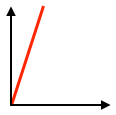
\includegraphics{img/plot1.png}
\caption{Some data.\label{fig:data}}
\end{figure}

\begin{figure}[htbp]
\centering
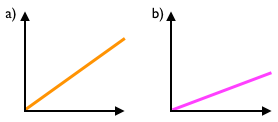
\includegraphics{img/plot2.png}
\caption{More data.\label{fig:more}}
\end{figure}

\renewcommand{\starnamesingular}{Figure}\Cref{fig:more}a and
\renewcommand{\plusnamesingular}{fig.}\cref{fig:more}b give more data.

\begin{figure}[htbp]
\centering
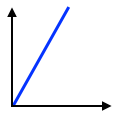
\includegraphics{img/plot3.png}
\caption{Even more
data.\label{fig:80412cec-d0c4-4c4c-86f8-87de2582a41d}}
\end{figure}
